\newpage
\section{Data Preparation}
%\begin{figure}[H]
%  \centering
%  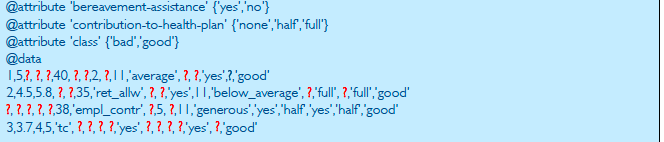
\includegraphics[width=.5\linewidth]{arffmissing}
%\end{figure}
Data preprocessing is important because the quality of data mining depends on the quality of the data . For example duplicates or missing values can lead to \textbf{wrong statistics} about the data. Data warehouses need \textbf{consistent integration} of quality data (it's actually the most time-consuming task in data warehouses).

\subsection{Data Cleaning}
\begin{itemize}
\item \textbf{Missing Values}\\
Values can missing because the information was \textbf{not collected} (e.g.: people not declaring age) or because attributes are  \textbf{not applicable} to all cases 
(e.g.: annual income not applicable to children).\\
These values can be \textbf{eliminated}, \textbf{imputated} , \textbf{ignored}...
\item \textbf{Duplicate data}\\
Dataset may include duplicate data or almost duplicates of one another.This can be an \textbf{issue} when \textbf{merging data} from heterogeneous source (e.g. : same person with multiple email addresses)
\item \textbf{Outliers}\\
Outliers are data objects with characteristics that are considerably different than most of the other data objects in the dataset.
\end{itemize}

\subsection{Sampling}
Sampling is the main data technique used for \textbf{data selection}. It is used in the \textbf{preliminary phase} of investigation but also at the end, in the \textbf{final data analysis}.\\
Sampling is used because obtaining and processing the \textbf{entire dataset} of interest is \textbf{too expensive or time consuming} : it works well if the sample is \textbf{representative} ( = has approximately the same property) of the entire original data.
\begin{itemize}
\item \textbf{Simple Random Sampling} = equal probability of selecting any particular item
\item \textbf{Sampling without replacement} = as each item is selected, it is removed from the population
\item \textbf{Sampling with replacement} = objects are not removed and can be picked again (boostrap!)
\item \textbf{Stratified sampling} = split data into several \textbf{homogeneous} partitions, then draw random samples from partitions
\end{itemize}

\subsection{Aggregation}
Combining two or more attributes (or objects) into a \textbf{single attribute} (or object) . This helps to \textbf{reduce} the number of attributes or objects . Aggregation is also useful to introduce a \textbf{change of scale} : cities are aggregated into region, states ,countries ...for example.\\
Aggregated data is useful because it tends to be more \textbf{stable} , have less \textbf{variability}.

\subsection{Feature Creation}
Create \textbf{new } attributes that can capture \textbf{important informations} in a dataset ,much more efficiently than the original attributes (e.g.: given an address create longitude and latitude attributes).
The main operations that can be done to create new features:
\begin{itemize}
\item \textbf{Feature extraction}
\item \textbf{Mapping data to a new space}
\item \textbf{Feature construction} (combining features)
\end{itemize}

\subsection{Discretization}
Attributes can be :
\begin{itemize}
\item \textbf{Nominal} : values from \textbf{unordered set}.
\item \textbf{Ordinal} : values from \textbf{ordered set}.
\item \textbf{Continuous}: real numbers.
\end{itemize}
The process of \textbf{discretization} consists of dividing \textbf{continuous} attributes in discrete intervals (some classification algorithms only accept \textbf{categorical} attributes!). This also reduces the data size and prepares data for future data analysis.\\
It can be done in two ways:
\begin{itemize}
\item \textbf{Supervised}\\
Attributes are discretized using \textbf{class information}. This methods tries to minimize the loss of information about the class. Used for example in IR Classifier for classification rules. 
\item \textbf{Unsupervised}\\
Attributes are discretized solely based \textbf{on their values}.
\end{itemize}

\subsection{Feature Selection (Dimensionality Reduction)}
This step is required to avoid the \textbf{curse of dimensionality} , save amount of time and money required by data mining algorithms ,allow data to be visualized more easily and may help to eliminate irrelevant features or reduce noise.\\
Features may be \textbf{redundant} (duplicate all or almost all the information contained in one or more attributes) or \textbf{irrelevant} (contain no information that is useful for the data mining task).
\begin{itemize}
\item PCA
\item SVD
\item Other supervised / non-supervised techniques ...
\end{itemize}
Different \textbf{approaches} can be used:

\begin{itemize}

\item \textbf{Brute force} : try all possible subset of features as input to data mining algorithm

\item \textbf{Embedded approaches} : feature selection occurs naturally as part of data mining algorithm ( like lasso)

\item \textbf{Filter approaches} : features are selected using a procedure that is \textbf{independent} from a specific data mining algorithm , for example using a \textbf{correlation matrix}.

\item \textbf{Wrapper approaches}: use a data mining algorithm as a black box to find best subset of attributes (e.g.: genetic algorithm and decision tree to find best features of tree)
\end{itemize}


\subsubsection{Filter approach 1 : PCA}
PCA is the \textbf{principal component analysis} which seeks a \textbf{basis} that best captures the \textbf{variance} in the data.This method works only on \textbf{numerical data}. The direction with the \textbf{largest} projected variance is called \textbf{first principal component}. The \textbf{orthogonal} direction that captures the \textbf{second largest} projected variance is the second principal component, and so on.\\
Goal is to find, given N data vectors from n-dimensions , \textbf{k}$<$ \textbf{n} orthogonal vectors:
\begin{enumerate}
\item \textbf{Normalize} input data
\item Compute k \textbf{orthonormal} vectors
\item Each input data vector is a \textbf{linear combination} of these components
\item The principal components are sorted in order of \textbf{decreasing significance}
\item Eliminate the \textbf{weak components} ( low explained variance)
\end{enumerate}
\begin{figure}[H]
  \centering
  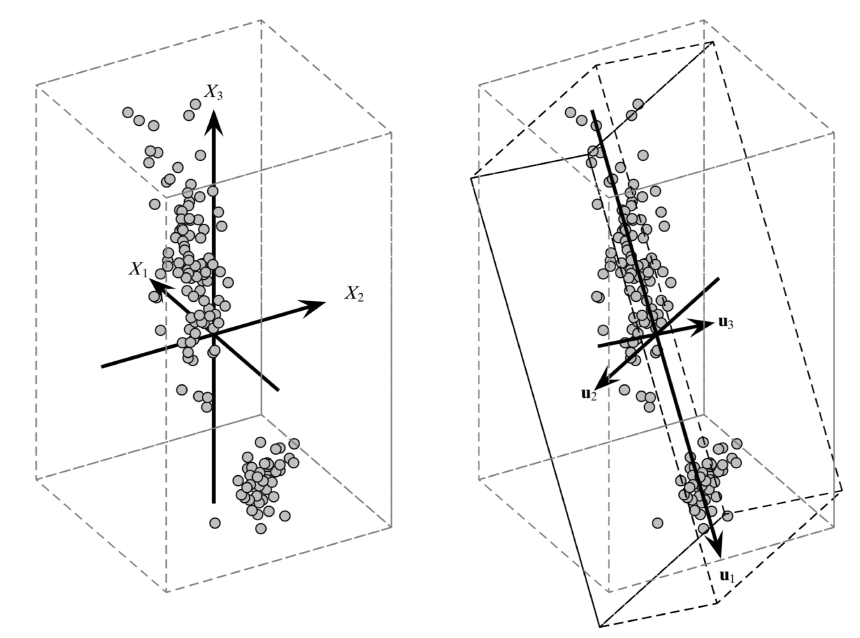
\includegraphics[width=.6\linewidth]{pca}
\end{figure}

\subsubsection{Filter approach 2 : SVD}
PCA is a special case of a more general \textbf{matrix decomposition} approach \textbf{Singular Value Decomposition} : it is \textbf{always} possible to decompose matrix \textbf{M} into $$ M= U \Sigma V^T$$
 where $U,\Sigma,V$ are \textbf{unique}.
 \begin{itemize}
 \item \textbf{U}:  is column orthonormal so that $UU^T = I$. This matrix represents the n samples using \textbf{r} new concepts/attributes
 \item $\Sigma$ : represents the \textbf{strength}  of each concept.$\Sigma_{i,j}$ are the \textbf{single values},positive and sorted in decreasing order.
 \item \textbf{V} : is column orthonormal so that $VV^T=I$. This matrix contains m terms, r concepts.
\end{itemize}  
\begin{figure}[H]
  \centering
  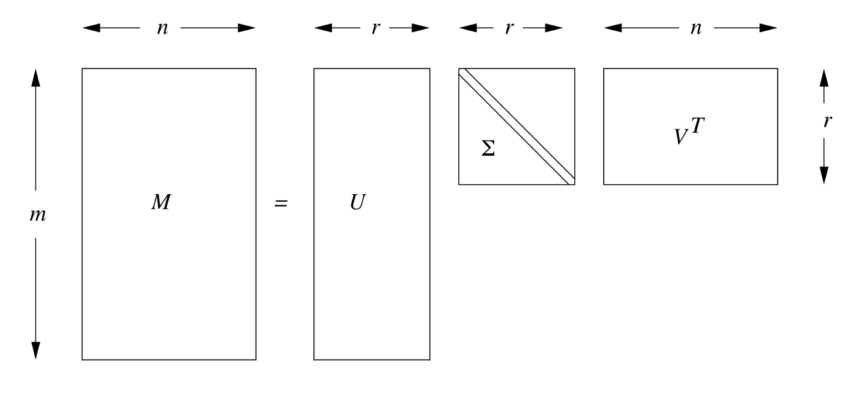
\includegraphics[width=.7\linewidth]{svd}
\end{figure}
An example:
\begin{figure}[H]
  \centering
  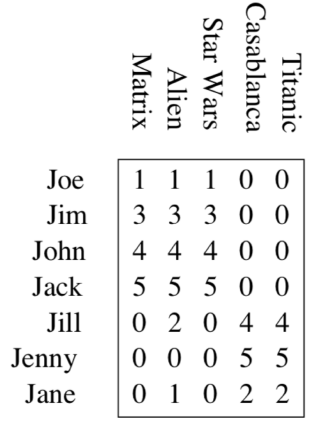
\includegraphics[width=.35\linewidth]{svd2}
\end{figure}
\begin{figure}[H]
  \centering
  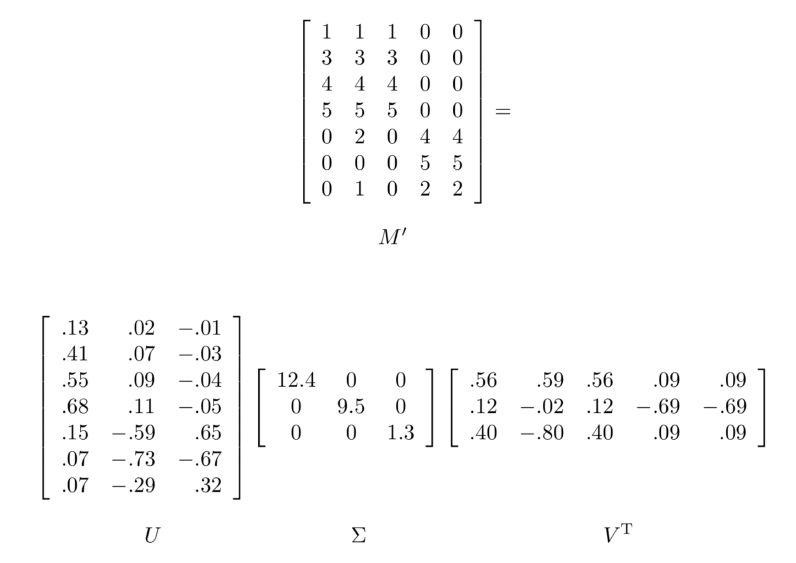
\includegraphics[width=.8\linewidth]{svd3}
\end{figure}
As seen in the $\Sigma$ matrix , which represents the \textbf{strength} of the concepts, the last column last row value $1.3$ is the weakest and could be eliminated (eliminating also the corresponding column in U and row in V).
\begin{figure}[H]
  \centering
  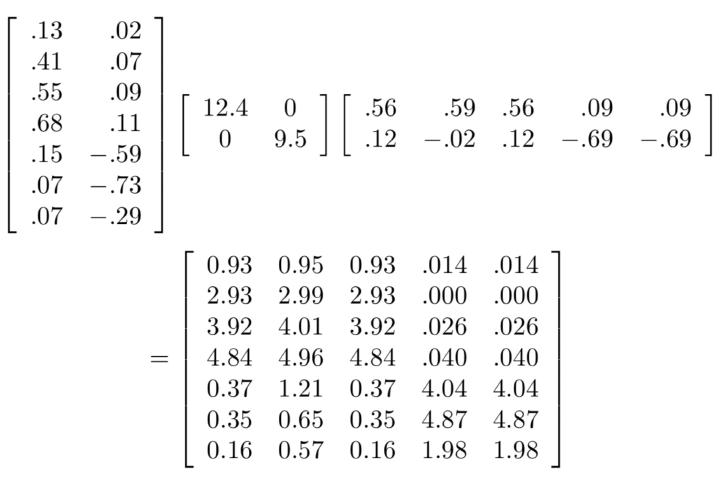
\includegraphics[width=.7\linewidth]{svd4}
\end{figure}
\textbf{How many singular values?}\\
Retain enough singular values to make up $90\%$ of the \textbf{energy} in $\Sigma$:
the \textbf{sum of squares} of the \textbf{retained} singular values should be at least $90\%$ of the energy of the singular values.\\
Example:
\begin{itemize}
\item $(12.4)^2 + (9.5)^2 + (1.3)^2 = 245.70$
\item $(12.4)^2 + (9.5)^2 = 244.01 \approx 99\%!$
\item $(12.4)^2 = 153.76 \approx 63\%$
\end{itemize}

\subsubsection{Wrapper Approach}
Focus on specific data mining algorithm and find the best subset of attributes for that specific algorithm . Example :find subset of features that maximizes DT performance. The algorithm is applied as a black box and uses a \textbf{search method} to find the best subset.
Different approaches:
\begin{itemize}
\item \textbf{Backward feature elimination}: start training on n input features, then remove one input at the time and train on n-1 input.\\
The input feature whose removal has produced the \textbf{smallest increase} in error rate is removed.\\
Each iteration k produces a model trained on n-k features and an error rate e(k). Stops when maximum tolerated error rate is reached.

\item \textbf{Forward feature creation}: inverse process of BFE.

\item \textbf{Recursively feature creation} : repeatedly creates a model and keeps aside the \textbf{best} and \textbf{worst} performing feature at each iteration. It construct the next model using the \textbf{remaining features} and then \textbf{ranks them} based on the order of elimination.
\end{itemize}


\subsubsection{Filter vs Wrapper}
\begin{itemize}
\item Filter approaches focus on the \textbf{relevance of features} while wrapper measure the \textbf{usefulness} of a subset of features by actually training a model
\item Filter approaches are faster since they do not require training ( wrappers are computationally expensive!)
\item Filter methods use \textbf{statistical methods} for evaluation while wrapper use \textbf{cross-validation}
\item Filter methods \textbf{fail} to find the \textbf{best subset} in many occasions while wrapper can \textbf{always} provide the best subset
\item Using the wrapper subset makes it more prone to overfitting!
\end{itemize}
